\documentclass[a4paper]{article}
\usepackage[utf8]{inputenc}
\usepackage{amsthm, amsmath, mathtools, amssymb}
\usepackage[left=1.5cm,right=1.5cm,top=1.5cm,bottom=1.5cm]{geometry}
\usepackage[colorlinks,linkcolor=blue,citecolor=blue,urlcolor=blue]{hyperref}
\usepackage{array}
\usepackage[catalan,english]{babel}
\usepackage[affil-it]{authblk}
\usepackage{titlesec}
\usepackage[intlimits]{esint} % for more options on integrals.
\usepackage{physics}
\usepackage[hypcap=false]{caption}
\usepackage{subcaption}
\usepackage{multirow}
\titleformat{\section}{\normalfont\fontsize{12}{14}\bfseries}{\thesection}{1em}{}

\newcommand{\NN}{\ensuremath{\mathbb{N}}} % set of natural numbers
\newcommand{\ZZ}{\ensuremath{\mathbb{Z}}} % set of integers
\newcommand{\QQ}{\ensuremath{\mathbb{Q}}} % set of rationals
\newcommand{\RR}{\ensuremath{\mathbb{R}}} % set of real numbers
\newcommand{\CC}{\ensuremath{\mathbb{C}}} % set of complex numbers
\newcommand{\KK}{\ensuremath{\mathbb{K}}} % a general field

\newcommand{\vf}[1]{\boldsymbol{\mathrm{#1}}} % math style for vectors and matrices and vector-values functions (previously it was \*vb{#1} but this does not apply to greek letters)
\newcommand{\ii}{\mathrm{i}} % imaginary unit
\renewcommand{\O}{\mathrm{O}} % big O-notation

\newtheorem{theorem}{Teorema}
\newtheorem{prop}{Proposició}
\theoremstyle{definition}
\newtheorem{definition}{Definició}
\DeclareDocumentCommand\derivative{ s o m g d() }{ 
  % Total derivative
  % s: star for \flatfrac flat derivative
  % o: optional n for nth derivative
  % m: mandatory (x in df/dx)
  % g: optional (f in df/dx)
  % d: long-form d/dx(...)
    \IfBooleanTF{#1}
    {\let\fractype\flatfrac}
    {\let\fractype\frac}
    \IfNoValueTF{#4}
    {
        \IfNoValueTF{#5}
        {\fractype{\diffd \IfNoValueTF{#2}{}{^{#2}}}{\diffd #3\IfNoValueTF{#2}{}{^{#2}}}}
        {\fractype{\diffd \IfNoValueTF{#2}{}{^{#2}}}{\diffd #3\IfNoValueTF{#2}{}{^{#2}}} \argopen(#5\argclose)}
    }
    {\fractype{\diffd \IfNoValueTF{#2}{}{^{#2}} #3}{\diffd #4\IfNoValueTF{#2}{}{^{#2}}}\IfValueT{#5}{(#5)}}
} % differential operator
\DeclareDocumentCommand\partialderivative{ s o m g d() }{ 
  % Total derivative
  % s: star for \flatfrac flat derivative
  % o: optional n for nth derivative
  % m: mandatory (x in df/dx)
  % g: optional (f in df/dx)
  % d: long-form d/dx(...)
  \IfBooleanTF{#1}
    {\let\fractype\flatfrac}
    {\let\fractype\frac}
    \IfNoValueTF{#4}{
      \IfNoValueTF{#5}
      {\fractype{\partial \IfNoValueTF{#2}{}{^{#2}}}{\partial #3\IfNoValueTF{#2}{}{^{#2}}}}
      {\fractype{\partial \IfNoValueTF{#2}{}{^{#2}}}{\partial #3\IfNoValueTF{#2}{}{^{#2}}} \argopen(#5\argclose)}
    }
    {\fractype{\partial \IfNoValueTF{#2}{}{^{#2}} #3}{\partial #4\IfNoValueTF{#2}{}{^{#2}}}\IfValueT{#5}{(#5)}}
} % partial differential operator

\renewcommand{\labelenumii}{\alph{enumii})}

\title{\bfseries\large SEMINARI 3\\\vspace{0.25cm}Òrbites periòdiques en semi-sistemes dinàmics discrets 1-dimensionals}

\author{Víctor Ballester Ribó\endgraf NIU:1570866\\(amb co\lgem aboració de Miquel Nasarre)}
\date{\parbox{\linewidth}{\centering
  Sistemes dinàmics\endgraf
  Grau en Matemàtiques\endgraf
  Universitat Autònoma de Barcelona\endgraf
  Febrer de 2023}}

\setlength{\parindent}{0pt}
\begin{document}
\selectlanguage{catalan}
\maketitle
L'objectiu d'aquest seminari és estudiar el comportament de les òrbites periòdiques d'alguns semi-sistemes dinàmics discrets en una dimensió. En les funcions $f_\mu(x)$ que hi ha a continuació calcularem primer de tot els valors $\mu_k$ tal que $\mu=\mu_k$ és la primera vegada que apareix el període $2^k$. Amb aquests valors intentarem predir el límit de la successió $(\lambda_k)$ on $$\lambda_k=\frac{\mu_{k-1}-\mu_{k-2}}{\mu_{k}-\mu_{k-1}}$$ A més, també calcularem els valors de $\mu$ pels que apareixen per primera vegada els períodes 7, 5 i 3, que són els últims en aparèixer segons el teorema de Sharkovskii. Finalment, farem el gràfic del diagrama de bifurcació $(\mu, x)$ en cada cas.

En tots els casos per tal de calcular els punts del paràmetre $\mu$ on apareixen les bifurcacions hem usat el mètode de Newton 2-dimensional fent derivació numèrica, com s'explica a continuació.
Com que en general volem calcular els zeros d'una funció de la forma $\vf{F}(x, \mu) = ({f_\mu}^n - x, {({f_\mu}^n)}_x \pm 1)$, necessitem saber la diferencial $\vf{DF}(x,\mu)$. Per això, si denotem $g(x,\mu):={({f_\mu}^n)}(x)$ necessitem saber les derivades ${g}_x$, ${g}_\mu$, ${g}_{xx}$ i ${g}_{x\mu}$, que les podem obtenir a partir de les fórmules següents:
\begin{align*}
  g_x(x,\mu)      & =\frac{g(x+h,\mu)-g(x-h,\mu)}{2h} + \O(h^2)                                 \\
  g_\mu(x,\mu)    & =\frac{g(x,\mu+h)-g(x,\mu-h)}{2h} + \O(h^2)                                 \\
  g_{xx}(x,\mu)   & =\frac{g(x+h,\mu)-2g(x,\mu)+g(x-h,\mu)}{h^2} + \O(h^2)                      \\
  g_{x\mu}(x,\mu) & =\frac{g(x+h,\mu+h)-g(x-h,\mu+h)-g(x+h,\mu-h)+g(x-h,\mu-h)}{4h^2} + \O(h^2) \\
\end{align*}
Notem que aquestes fórmules s'obtenen directament de l'expressió en sèrie de potències de $g$. Les condicions inicials per el mètode les podem obtenir graficant la funció i observant (molt aproximadament) on hi ha el zero de $g$.

També se'ns demana que donem en cada cas valors de $\mu$ tal que aparegui un cert període però no un altre. Això és una conseqüència immediata del teorema de Sharkovskii, que ens assegura que podem triar qualsevol dels $\mu$'s continguts en l'interval amb extrems els dos valors de $\mu$ tals que apareixen per primera vegada tals períodes i de manera que l'extrem esquerra de l'interval correspon al període més petit en l'ordre de Sharkovskii.
Dit això, a continuació s'exposen els resultats obtinguts:
\newpage
\section{\texorpdfstring{$\boldsymbol{f_\mu(x)=\mu x(1-x)\quad x\in[0,1], \mu\in[0,4]}$}{f1}}
A la següent taula mostrem els valors aproximats de $\mu_k$ i $\lambda_k$ per a valors de $k$ petits:
\begin{table}[ht]
  \centering
  \begin{tabular}{c|c|c}
    $k$ & $\mu_k$  & $\lambda_k$ \\
    \hline
    \hline
    1   & 3.000000 & -           \\
    2   & 3.449490 & -           \\
    3   & 3.544090 & 4.751446    \\
    4   & 3.564407 & 4.656251    \\
    5   & 3.568759 & 4.668242    \\
    6   & 3.569692 & 4.668739    \\
    7   & 3.569891 & 4.669132    \\
    8   & 3.569934 & 4.669183    \\
    9   & 3.569943 & 4.669198    \\
    10  & 3.569945 & 4.669201    \\
    11  & 3.569946 & 4.669201
  \end{tabular}
\end{table}

A més la primera vegada que apareixen els períodes 7, 5 i 3 són respectivament en $\mu = 3.701641$, $\mu= 3.738172$ i $\mu = 3.828427$.
Els gràfics següents mostren les aparicions d'alguns dels períodes així com el diagrama de bifurcació de la funció.
\begin{figure}[ht]
  \begin{subfigure}[ht]{0.45\linewidth}
    \centering
    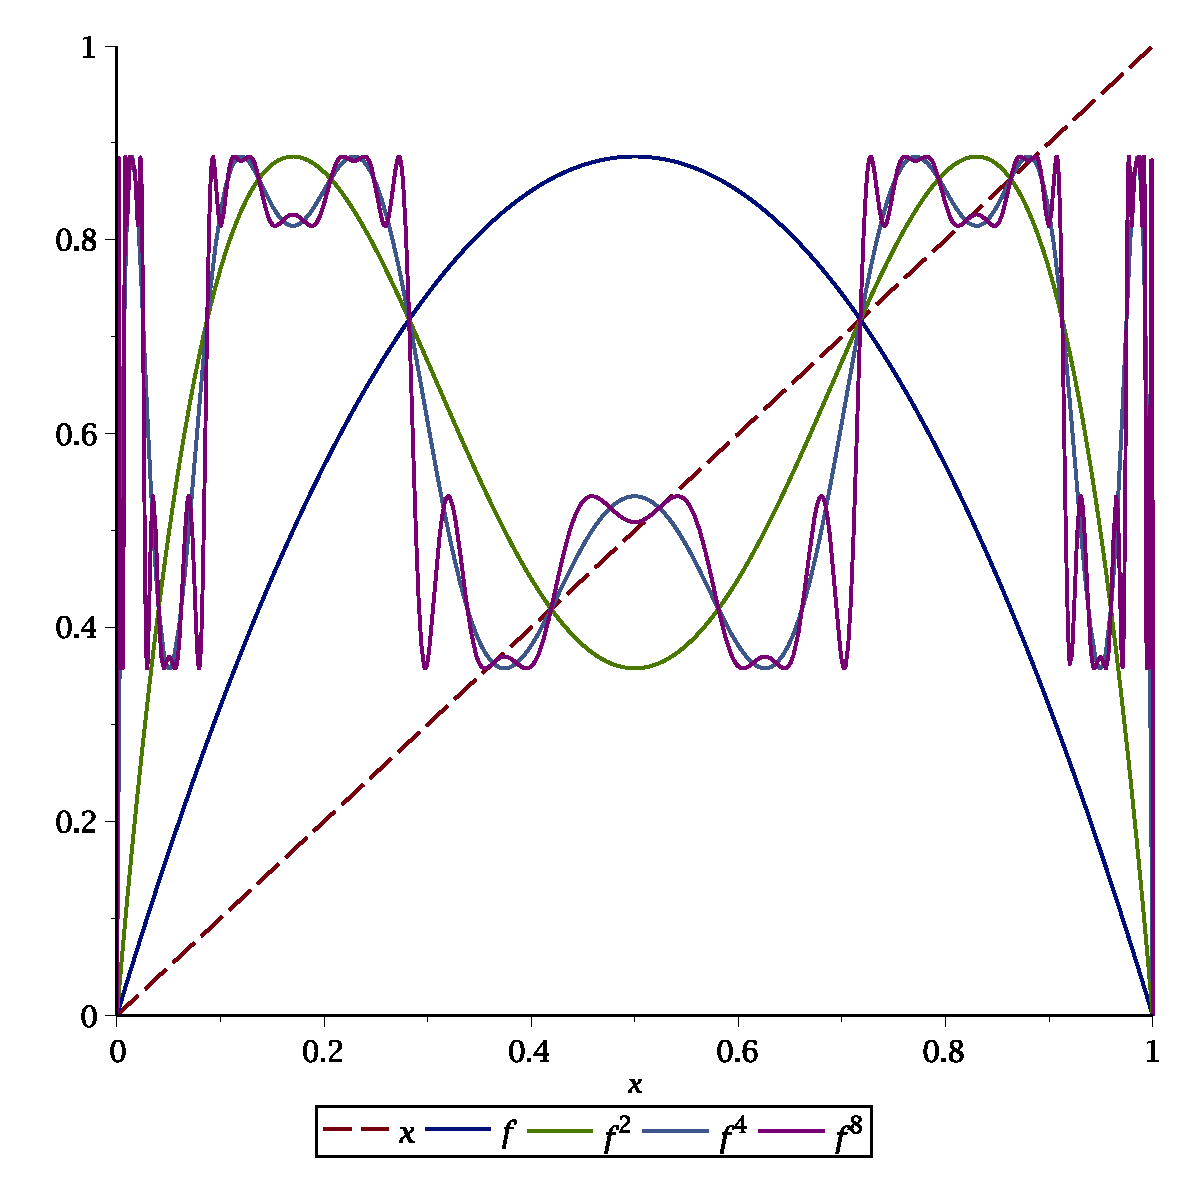
\includegraphics[width=\linewidth]{Images/map12.eps}
    \caption{Aparició del període 8}
  \end{subfigure}
  \hfill
  \begin{subfigure}[ht]{0.45\linewidth}
    \centering
    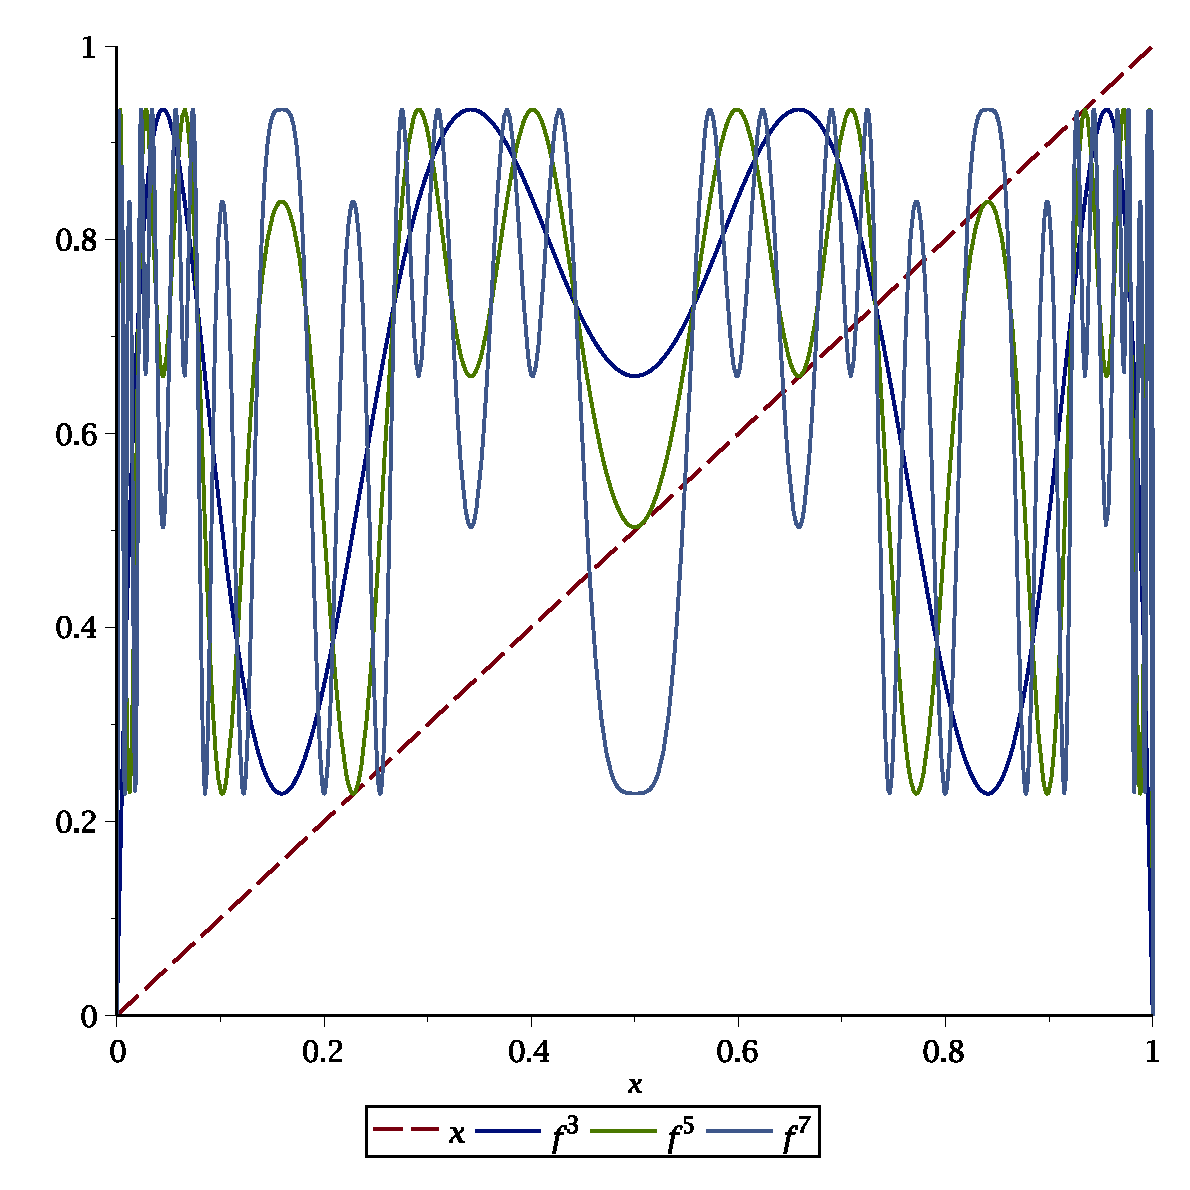
\includegraphics[width=\linewidth]{Images/map15.eps}
    \caption{Aparició del període 5}
  \end{subfigure}
\end{figure}
\begin{center}
  \begin{minipage}{\linewidth}
    \centering
    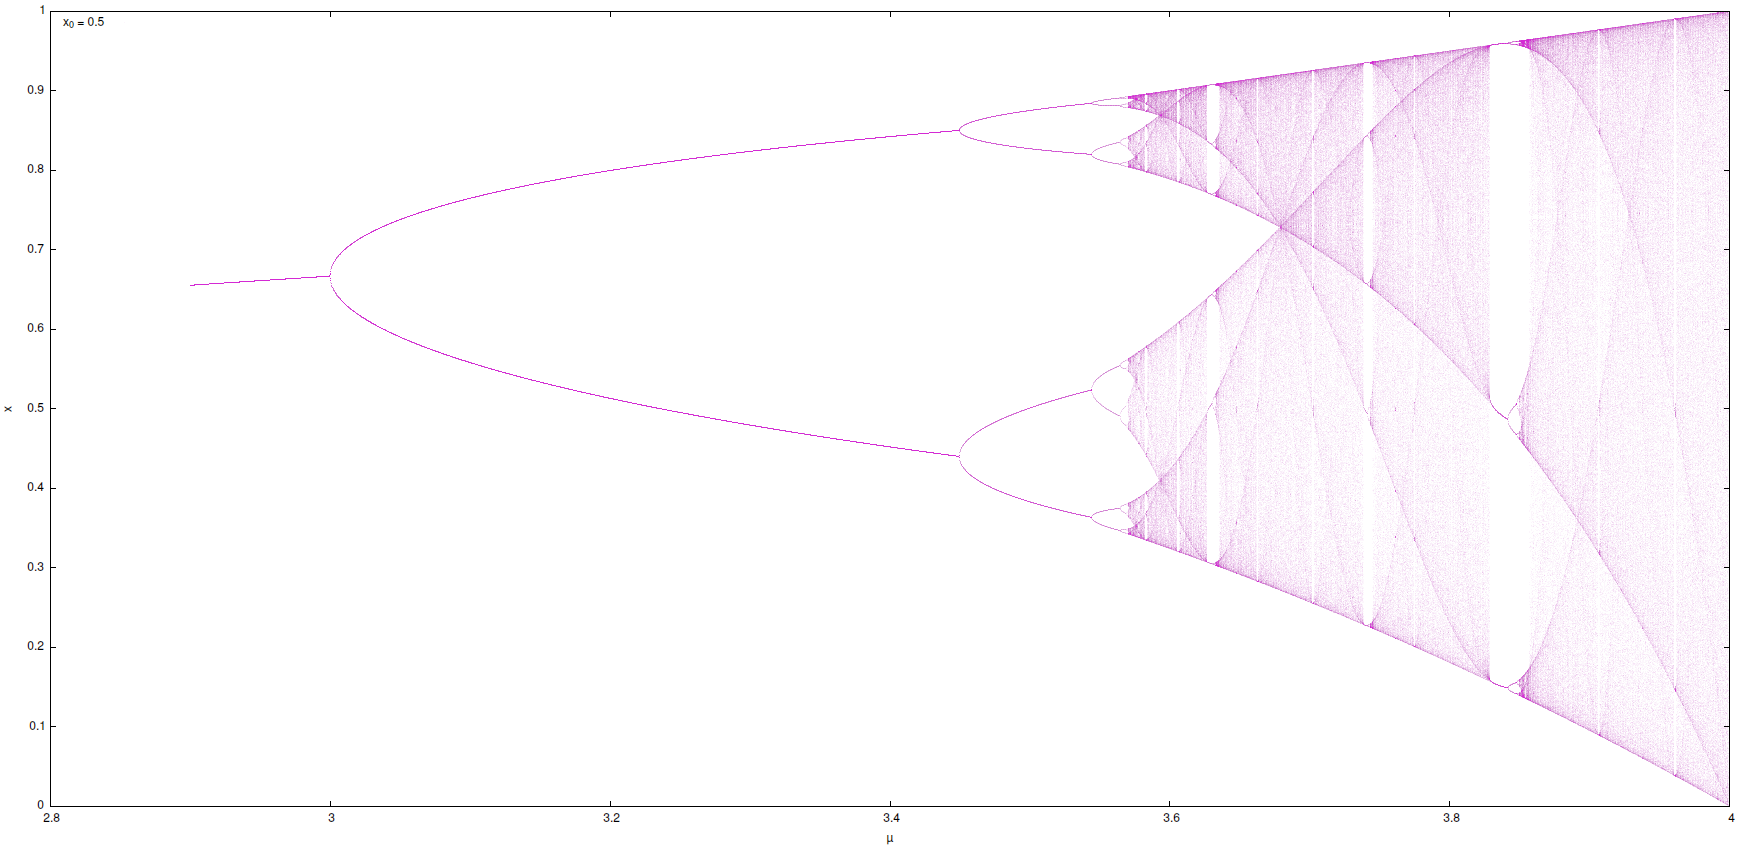
\includegraphics[width=0.8\linewidth]{Images/map1.png}
    \captionof{figure}{Diagrama de bifurcació de la iteració $f_\mu(x)=\mu x(1-x)$ començant en $x=0.5$}
  \end{minipage}
\end{center}
Notem a més que la silueta general del dibuix és independent del valor inicial on comencem.

\newpage
\section{\texorpdfstring{$\boldsymbol{f_\mu(x)=\mu x\frac{1-x}{1+x}\quad x\in[0,1], \mu\in[0,3+2\sqrt{2}]}$}{f2}}
A la següent taula mostrem els valors aproximats de $\mu_k$ i $\lambda_k$ per a valors de $k$ petits:
\begin{table}[ht]
  \centering
  \begin{tabular}{c|c|c}
    $k$ & $\mu_k$  & $\lambda_k$ \\
    \hline
    \hline
    1   & 4.236068 & -           \\
    2   & 5.027339 & -           \\
    3   & 5.184932 & 5.020989    \\
    4   & 5.218761 & 4.658527
  \end{tabular}
\end{table}

A més la primera vegada que apareixen els períodes 7, 5 i 3 són respectivament en $\mu = 5.457522$, $\mu= 5.515016$ i $\mu = 5.641364$.

El problema de calcular els punts de bifurcació amb aquesta funció està bastant mal condicionat i és per això que, tot i que es podrien haver donat més valors amb una mica més d'esforç, he decidit no donar-ne més per contrastar la dificultat en comparació amb les altres functions.

Els gràfics següents mostren les aparicions d'alguns dels períodes així com el diagrama de bifurcació de la funció.
\begin{figure}[ht]
  \begin{subfigure}[ht]{0.45\linewidth}
    \centering
    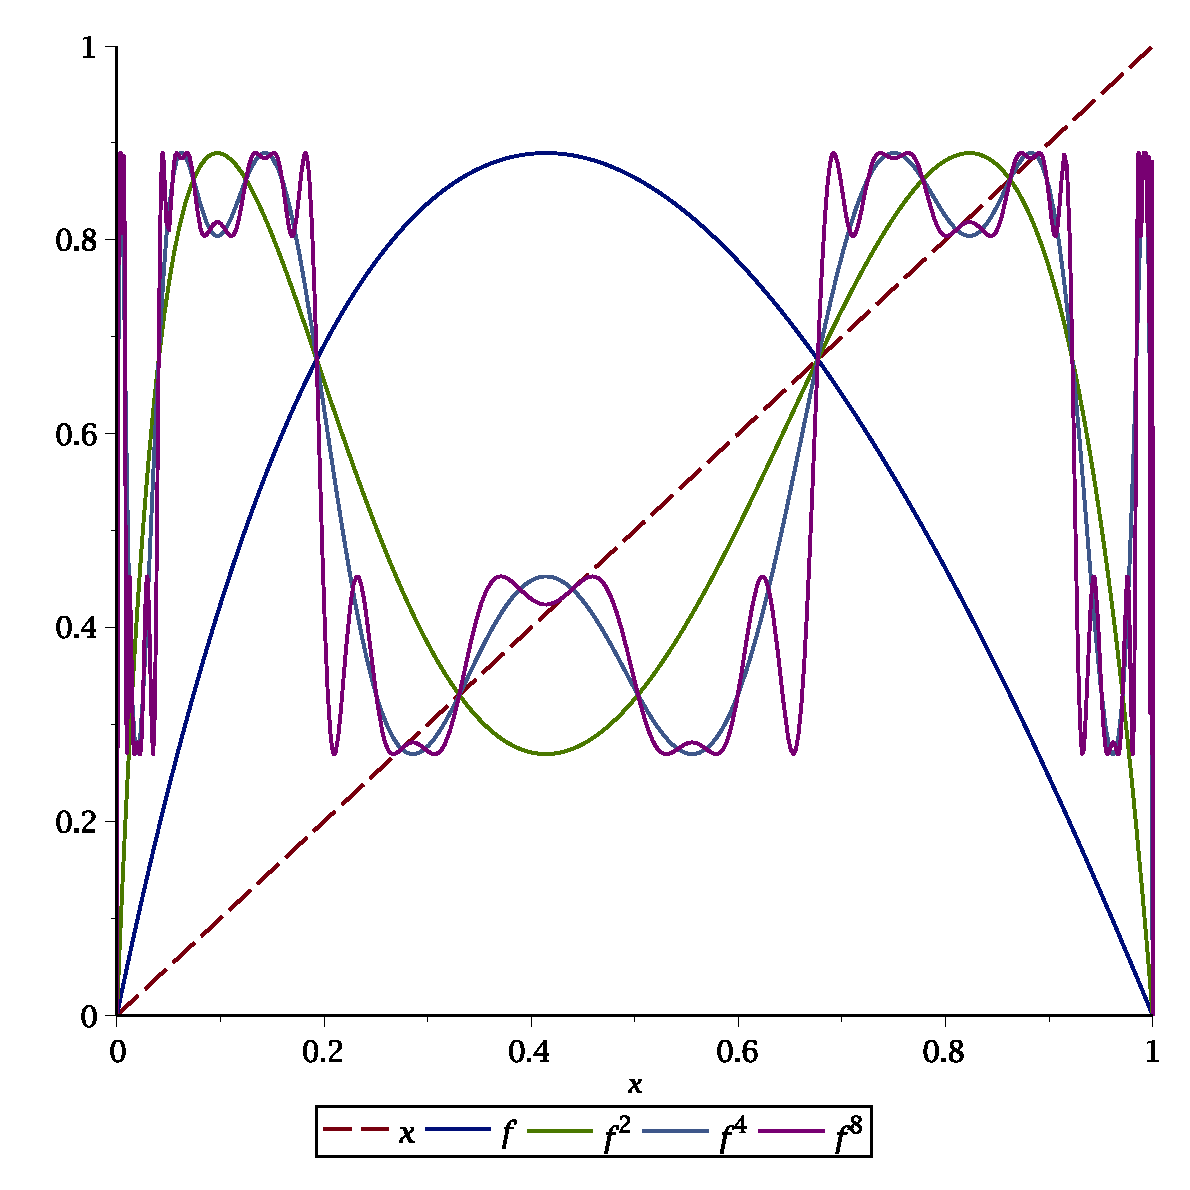
\includegraphics[width=\linewidth]{Images/map22.eps}
    \caption{Aparició del període 8}
  \end{subfigure}
  \hfill
  \begin{subfigure}[ht]{0.45\linewidth}
    \centering
    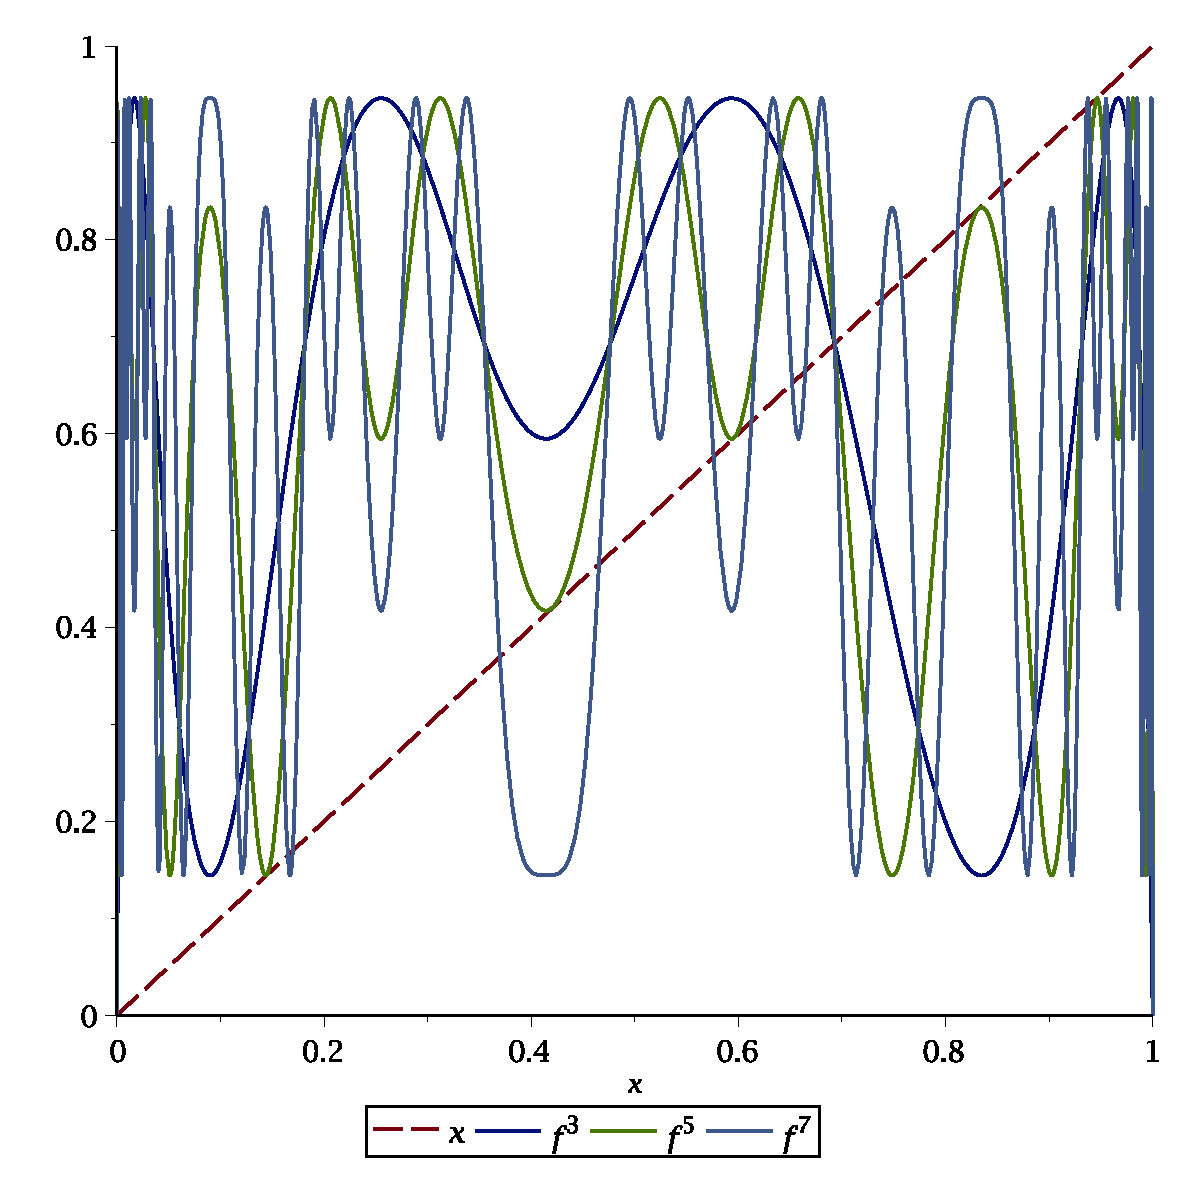
\includegraphics[width=\linewidth]{Images/map25.eps}
    \caption{Aparició del període 5}
  \end{subfigure}
\end{figure}
\begin{center}
  \begin{minipage}{\linewidth}
    \centering
    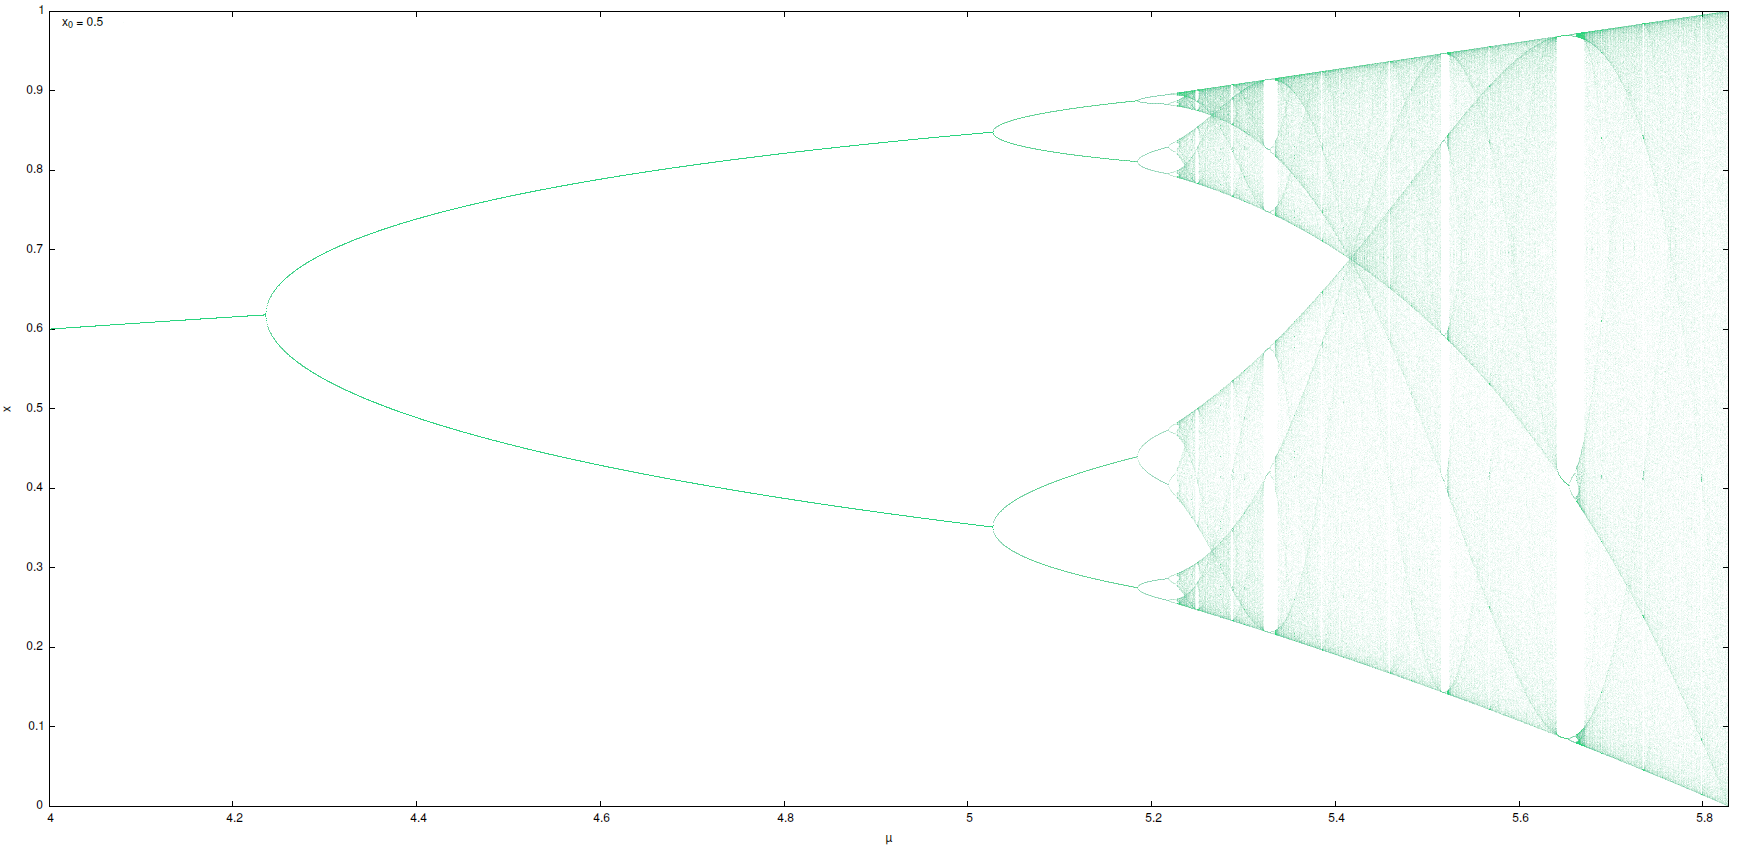
\includegraphics[width=0.8\linewidth]{Images/map2.png}
    \captionof{figure}{Diagrama de bifurcació de la iteració $f_\mu(x)=\mu x\frac{1-x}{1+x}$ començant en $x=0.5$}
  \end{minipage}
\end{center}

\newpage
\section{\texorpdfstring{$\boldsymbol{f_\mu(x)=\mu x(1-x^2)\quad x\in[0,1], \mu\in[0,3\sqrt{3}/2]}$}{f3}}
A la següent taula mostrem els valors aproximats de $\mu_k$ i $\lambda_k$ per a valors de $k$ petits:
\begin{table}[ht]
  \centering
  \begin{tabular}{c|c|c}
    $k$ & $\mu_k$  & $\lambda_k$ \\
    \hline
    \hline
    1   & 2.000000 & -           \\
    2   & 2.236068 & -           \\
    3   & 2.288032 & 4.542933    \\
    4   & 2.299228 & 4.641204    \\
    5   & 2.301629 & 4.663184
  \end{tabular}
\end{table}
A més la primera vegada que apareixen els períodes 7, 5 i 3 són respectivament en $\mu = 2.372987$, $\mu= 2.393925$ i $\mu =2.450441$.

De forma anàloga a la funció anterior, aquesta funció també propaga molt ràpidament els errors i amb el mètode de Newton es fa difícil (o si més no tediós) donar més valors de $\mu_k$ ja que ens hauríem d'apropar molt al valor real amb la condició inicial.

Els gràfics següents mostren les aparicions d'alguns dels períodes així com el diagrama de bifurcació de la funció.

\begin{figure}[ht]
  \begin{subfigure}[ht]{0.45\linewidth}
    \centering
    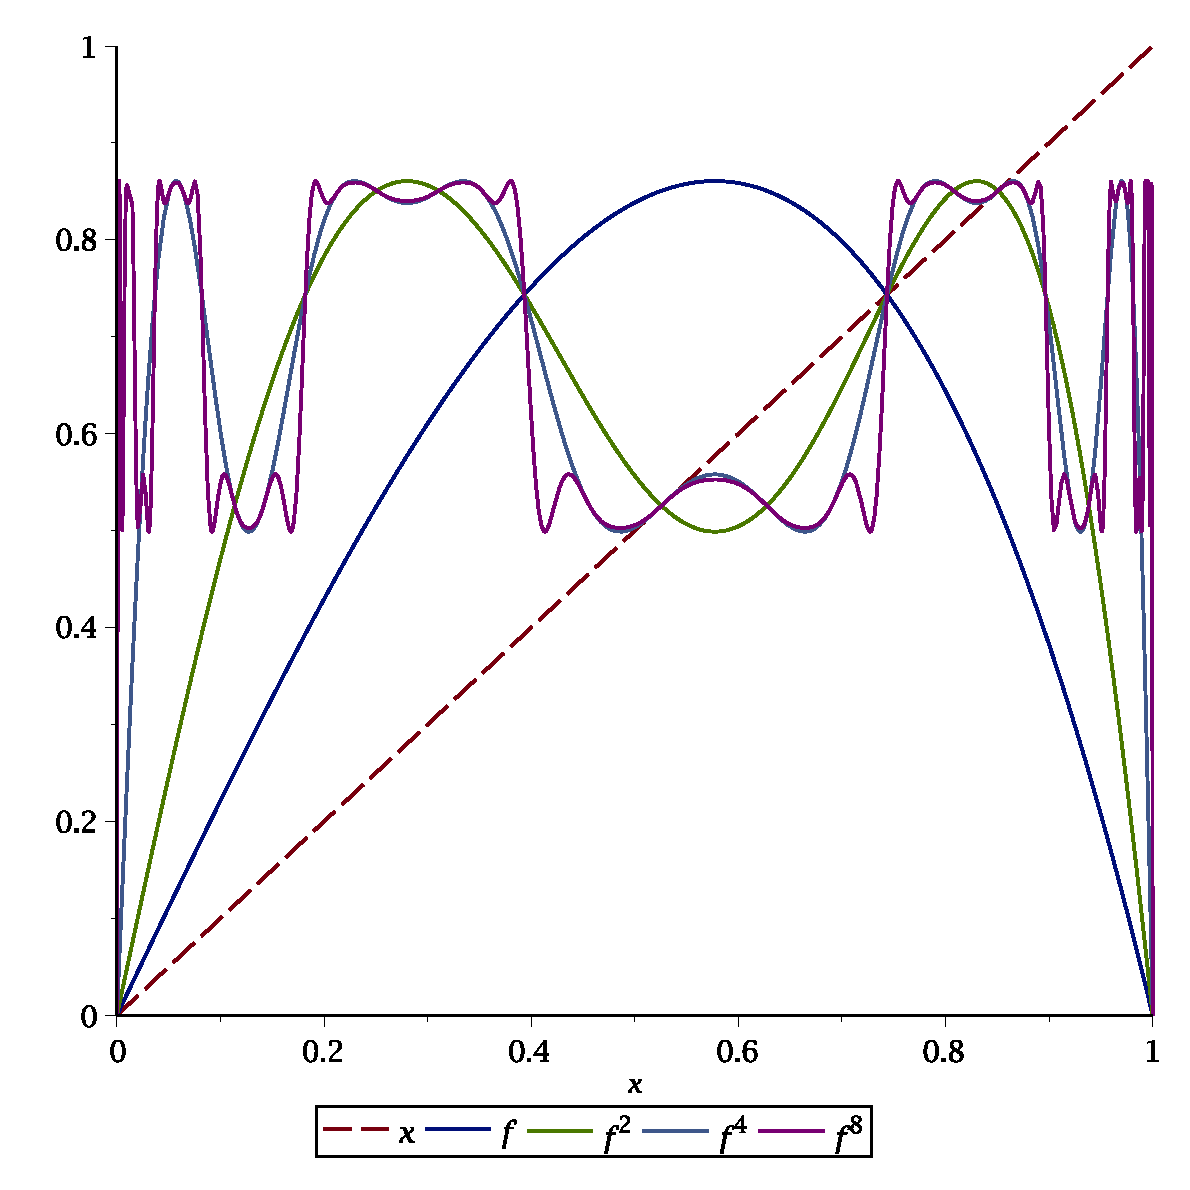
\includegraphics[width=\linewidth]{Images/map32.eps}
    \caption{Aparició del període 4}
  \end{subfigure}
  \hfill
  \begin{subfigure}[ht]{0.45\linewidth}
    \centering
    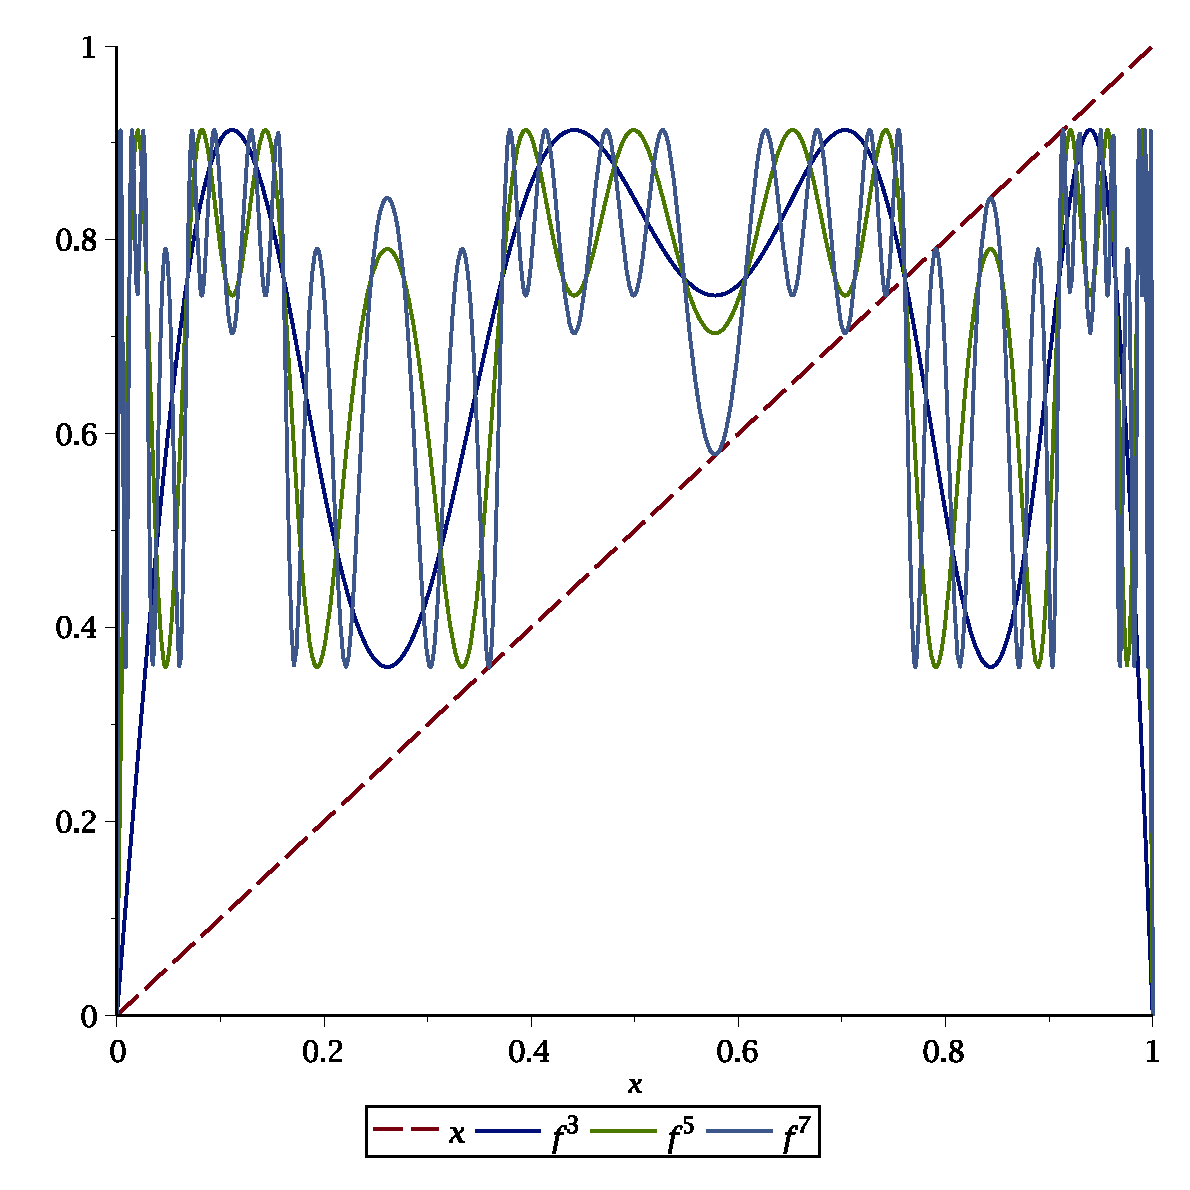
\includegraphics[width=\linewidth]{Images/map35.eps}
    \caption{Aparició del període 7}
  \end{subfigure}
\end{figure}
\begin{center}
  \begin{minipage}{\linewidth}
    \centering
    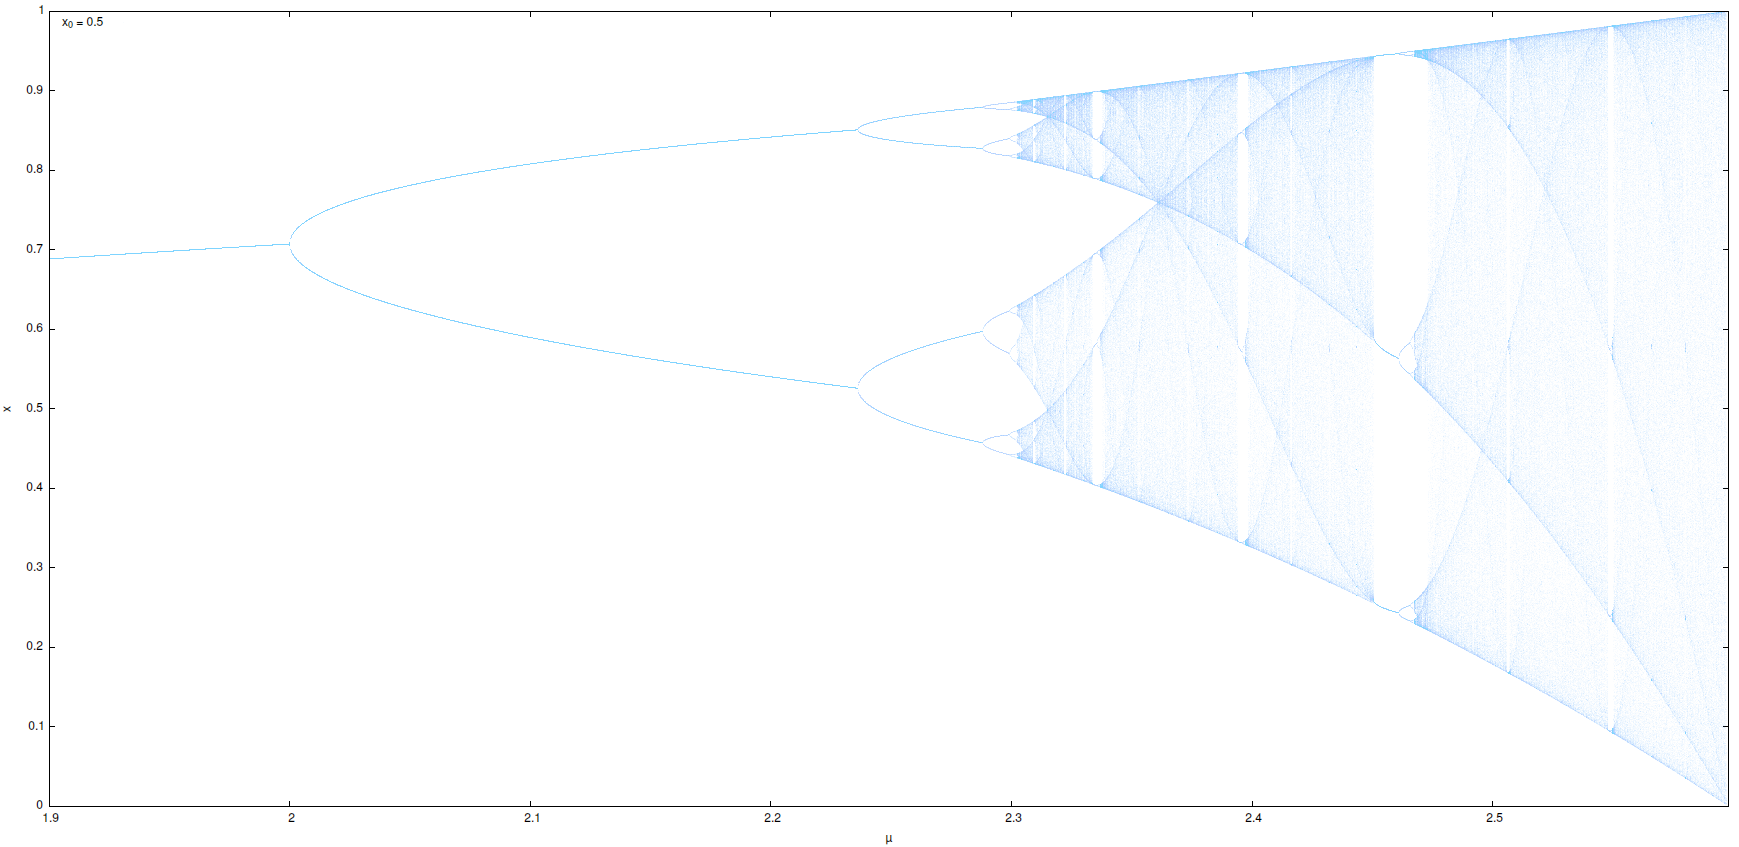
\includegraphics[width=0.8\linewidth]{Images/map3.png}
    \captionof{figure}{Diagrama de bifurcació de la iteració $f_\mu(x)=\mu x(1-x^2)$ començant en $x=0.5$}
  \end{minipage}
\end{center}
\newpage
\section{\texorpdfstring{$\boldsymbol{f_\mu(x)=\mu \cos(\pi x)\quad x\in[-1,1], \mu\in[0,1]}$}{f4}}

A la següent taula mostrem els valors aproximats de $\mu_k$ i $\lambda_k$ per a valors de $k$ petits:
\begin{table}[ht]
  \centering
  \begin{tabular}{c|c|c}
    $k$ & $\mu_k$  & $\lambda_k$ \\
    \hline
    \hline
    1   & 0.419901 & -           \\
    2   & 0.581575 & -           \\
    3   & 0.618440 & 4.385535    \\
    4   & 0.626260 & 4.714456    \\
    5   & 0.627931 & 4.678678    \\
    6   & 0.628289 & 4.671360    \\
    7   & 0.628366 & 4.669652    \\
    8   & 0.628382 & 4.669290    \\
    9   & 0.628386 & 4.669237    \\
    10  & 0.628387 & 4.669219
  \end{tabular}
\end{table}

A més la primera vegada que apareixen els períodes 7, 5 i 3 són respectivament en $\mu = 0.673974$, $\mu= 0.688820$ i $\mu = 0.734068$.
Els gràfics següents mostren les aparicions d'alguns dels períodes així com el diagrama de bifurcació de la funció.
\begin{figure}[ht]
  \begin{subfigure}[ht]{0.45\linewidth}
    \centering
    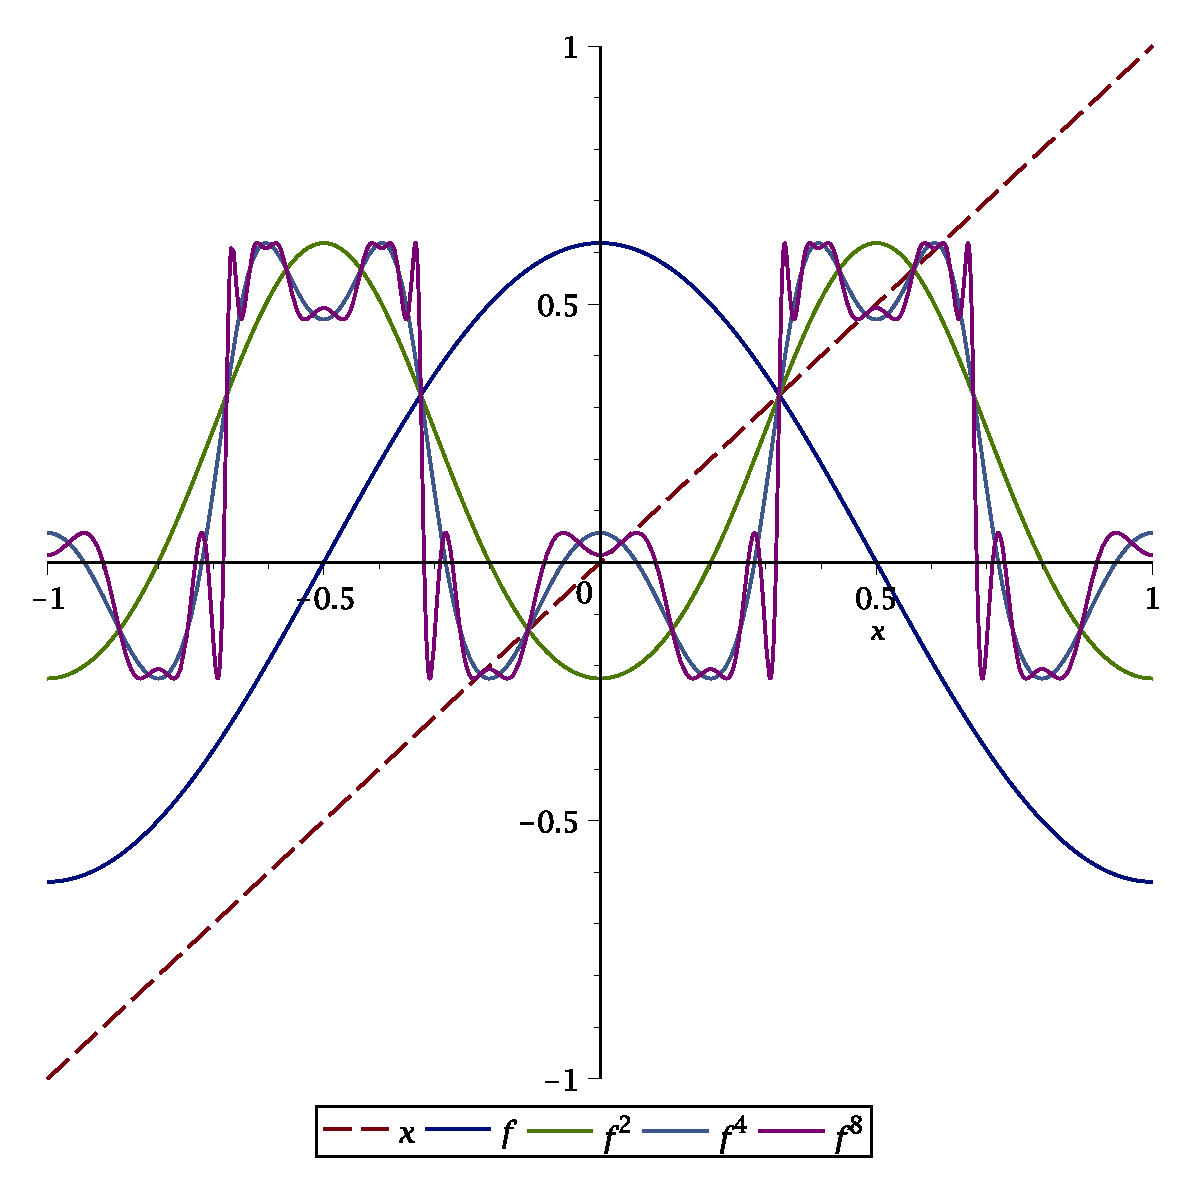
\includegraphics[width=\linewidth]{Images/map42.eps}
    \caption{Aparició del període 8}
  \end{subfigure}
  \hfill
  \begin{subfigure}[ht]{0.45\linewidth}
    \centering
    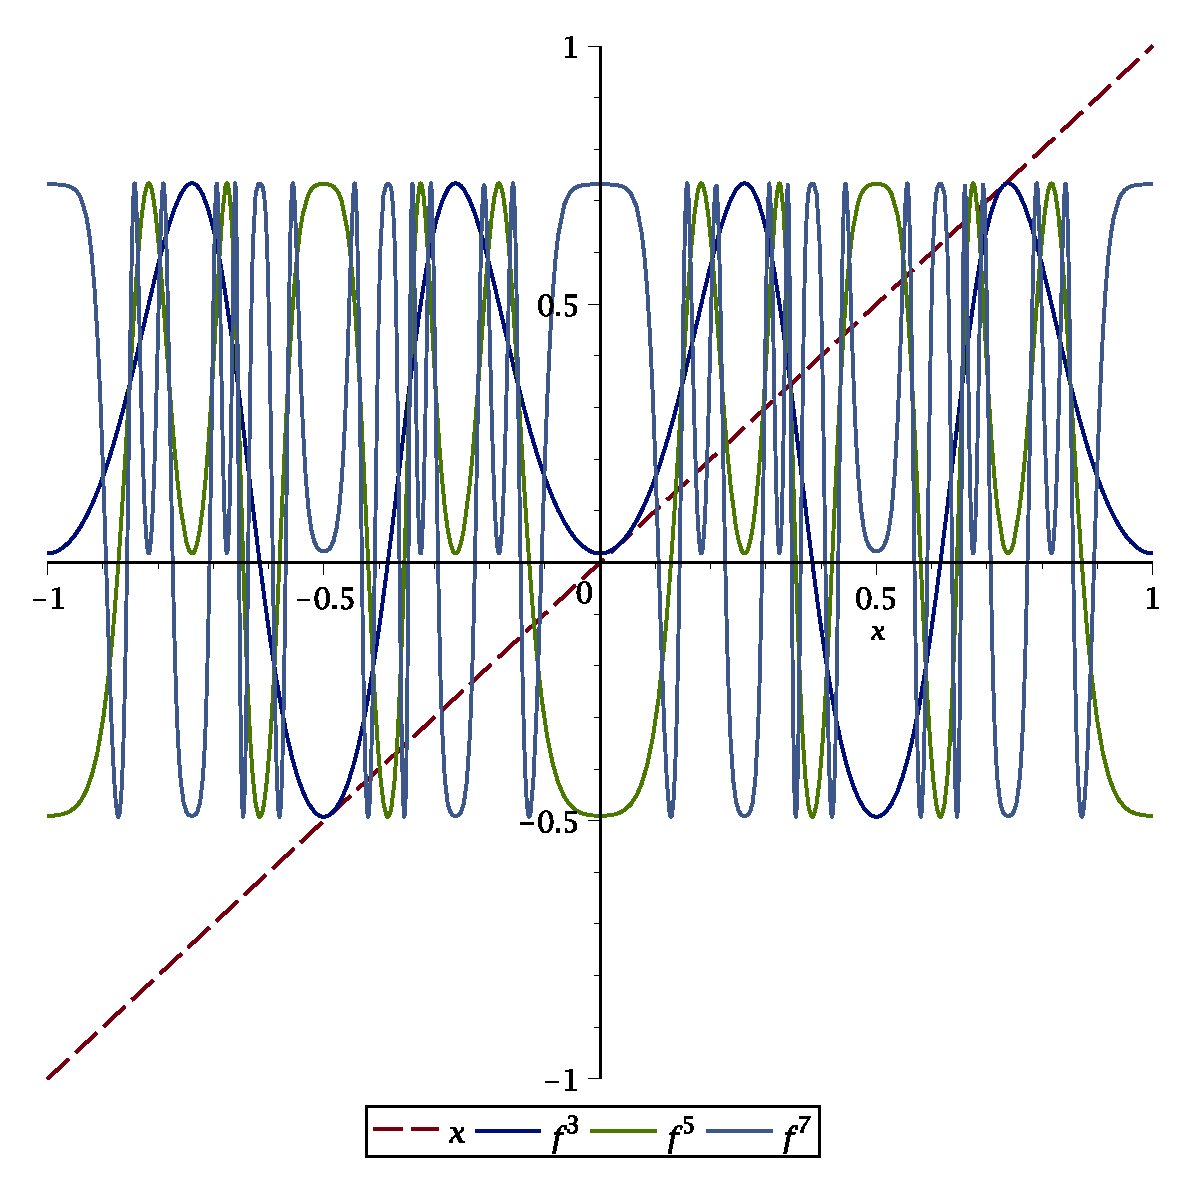
\includegraphics[width=\linewidth]{Images/map45.eps}
    \caption{Aparició del període 3}
  \end{subfigure}
\end{figure}
\begin{center}
  \begin{minipage}{\linewidth}
    \centering
    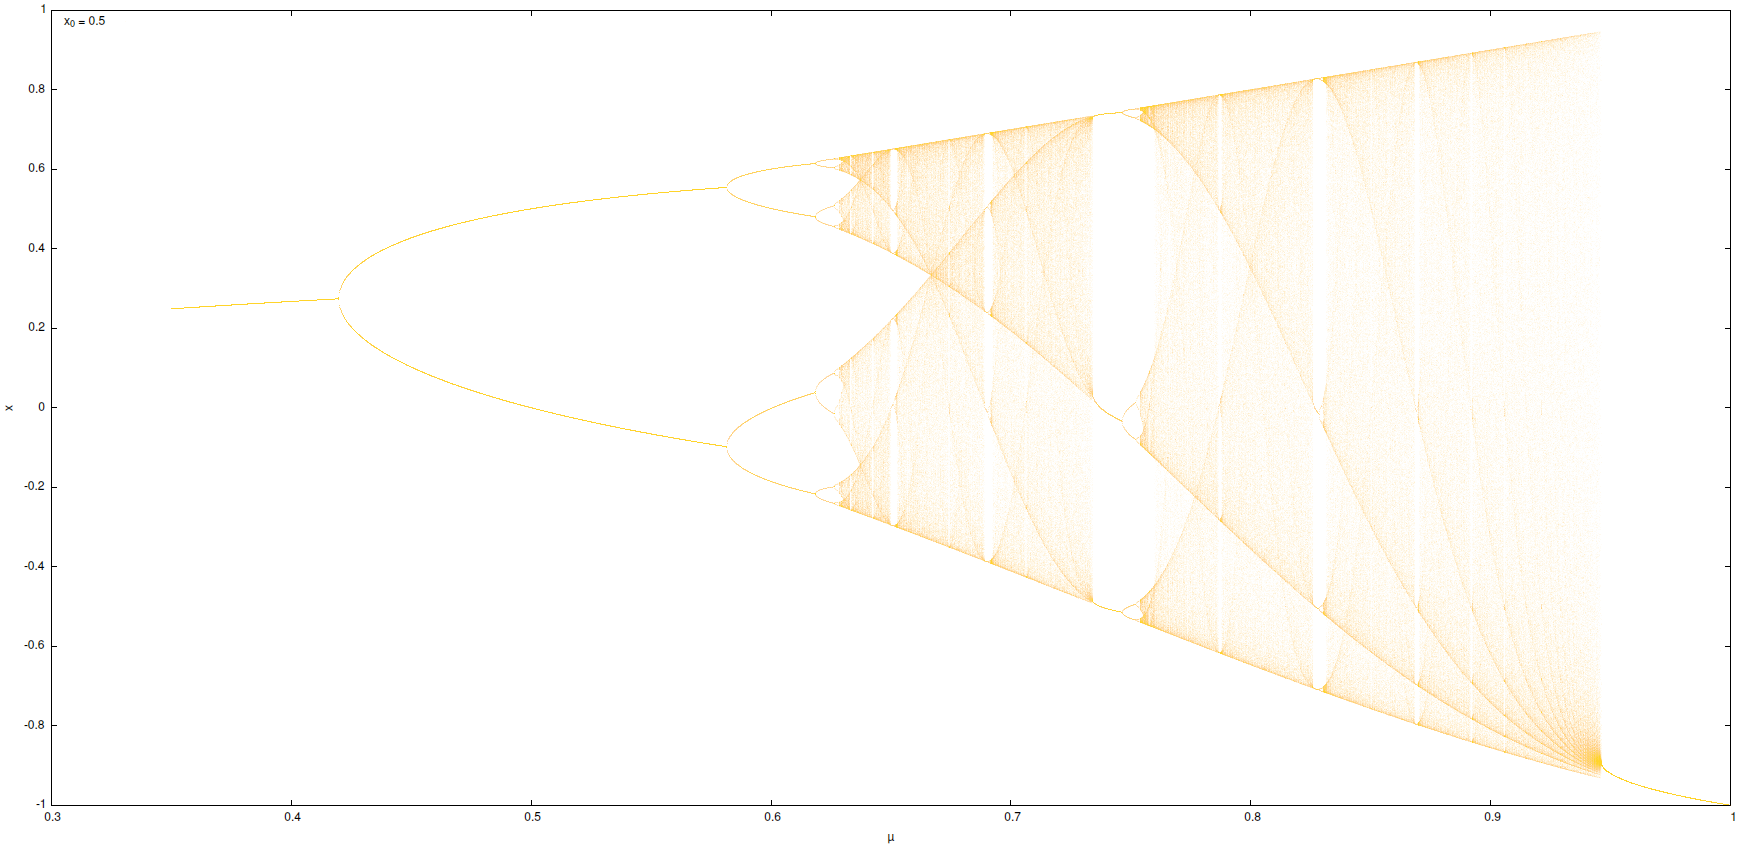
\includegraphics[width=0.8\linewidth]{Images/map4.png}
    \captionof{figure}{Diagrama de bifurcació de la iteració $f_\mu(x)=\mu \cos(\pi x)$ començant en $x=0.5$}
  \end{minipage}
\end{center}
\newpage
\section{\texorpdfstring{$\boldsymbol{f_\mu(x)=\begin{cases}
          \mu x    & x\in[0,1/2] \\
          \mu(1-x) & x\in[1/2,1]
        \end{cases}\quad \mu\in[0,2]}$}{f5}}
Els inconvenients del mètode de Newton fan que no sigui possible trobar els zeros d'aquesta funció no diferenciable. No obstant això podem veure la seva forma, en els gràfics següents així com el seu diagrama de bifurcació.
\begin{figure}[ht]
  \begin{subfigure}[ht]{0.45\linewidth}
    \centering
    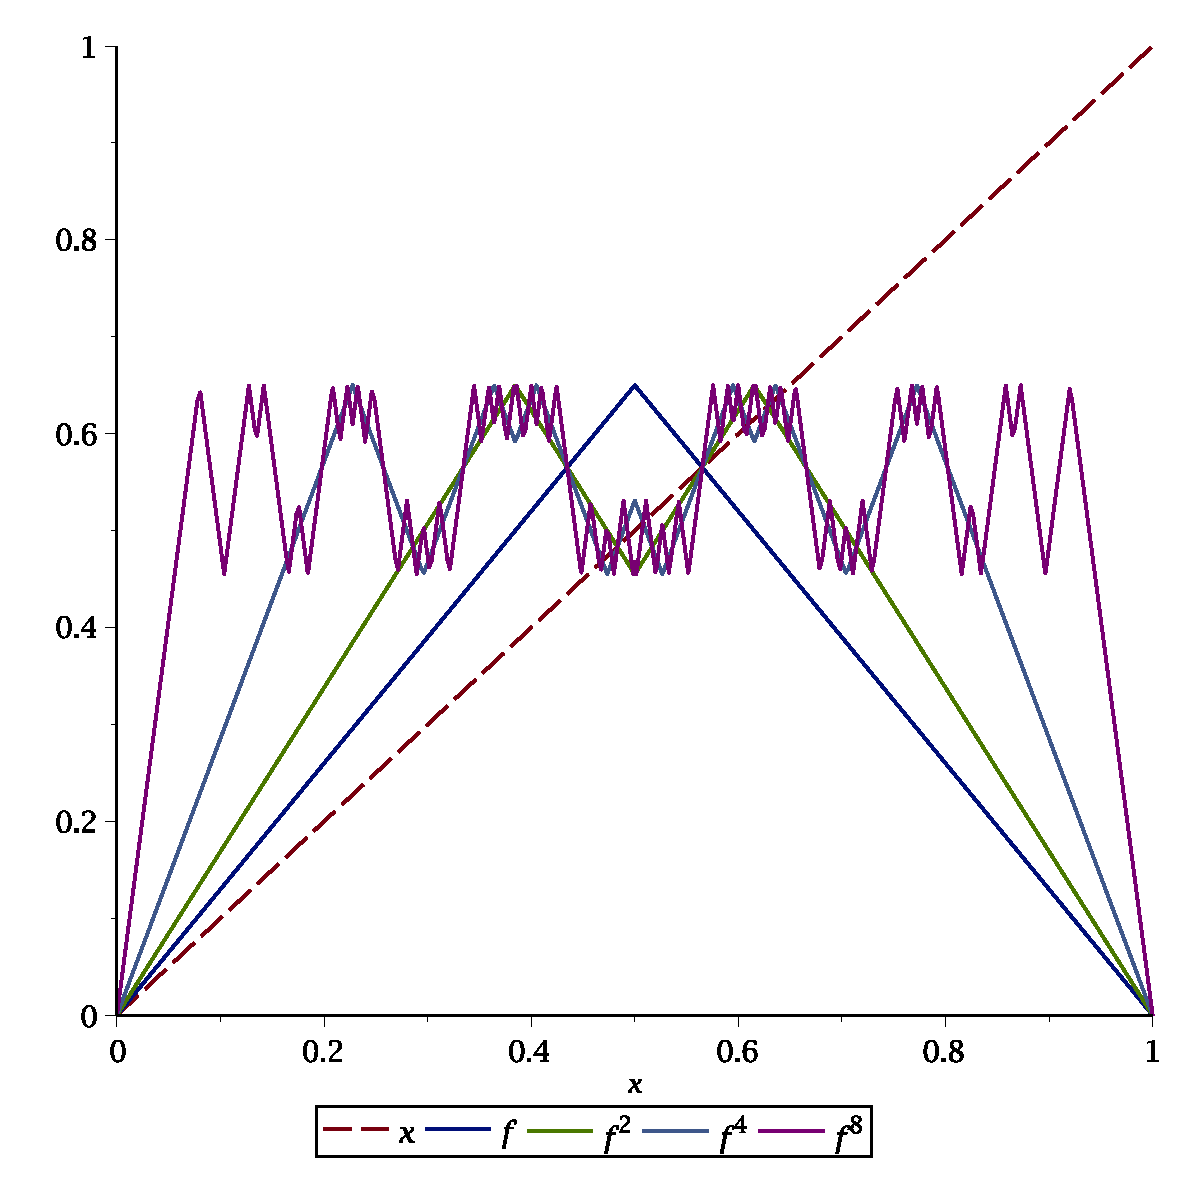
\includegraphics[width=\linewidth]{Images/map52.eps}
    \caption{Representació del les primeres iteracions de ${f_\mu }^n$}
  \end{subfigure}
  \hfill
  \begin{subfigure}[ht]{0.45\linewidth}
    \centering
    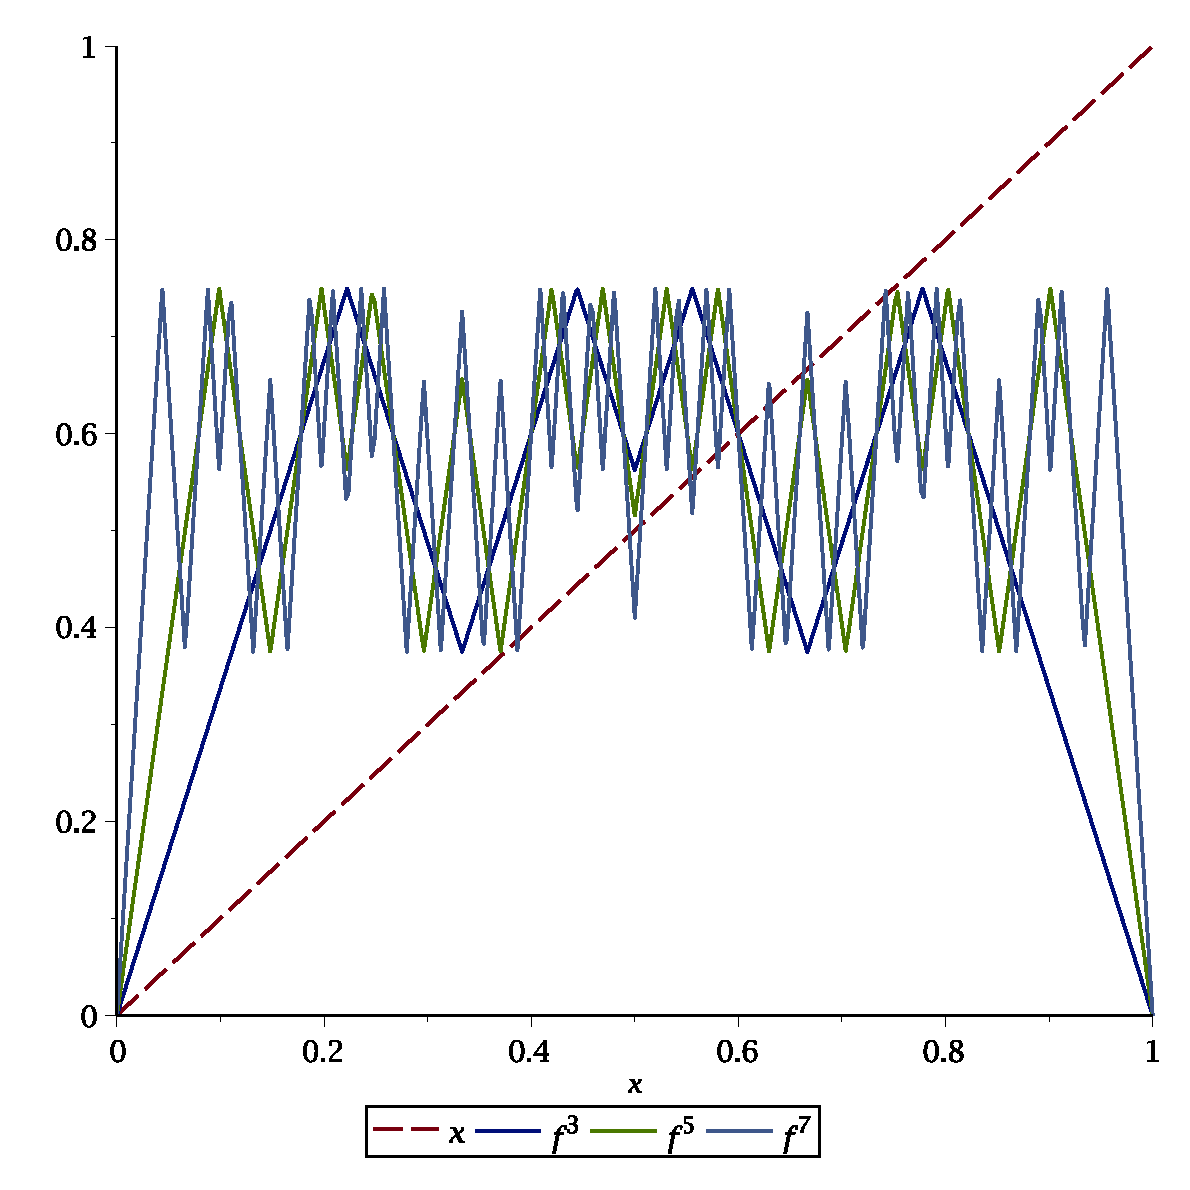
\includegraphics[width=\linewidth]{Images/map55.eps}
    \caption{Aproximació del naixement del període 5 quan $\mu = 1.5$}
  \end{subfigure}
\end{figure}
\begin{center}
  \begin{minipage}{\linewidth}
    \centering
    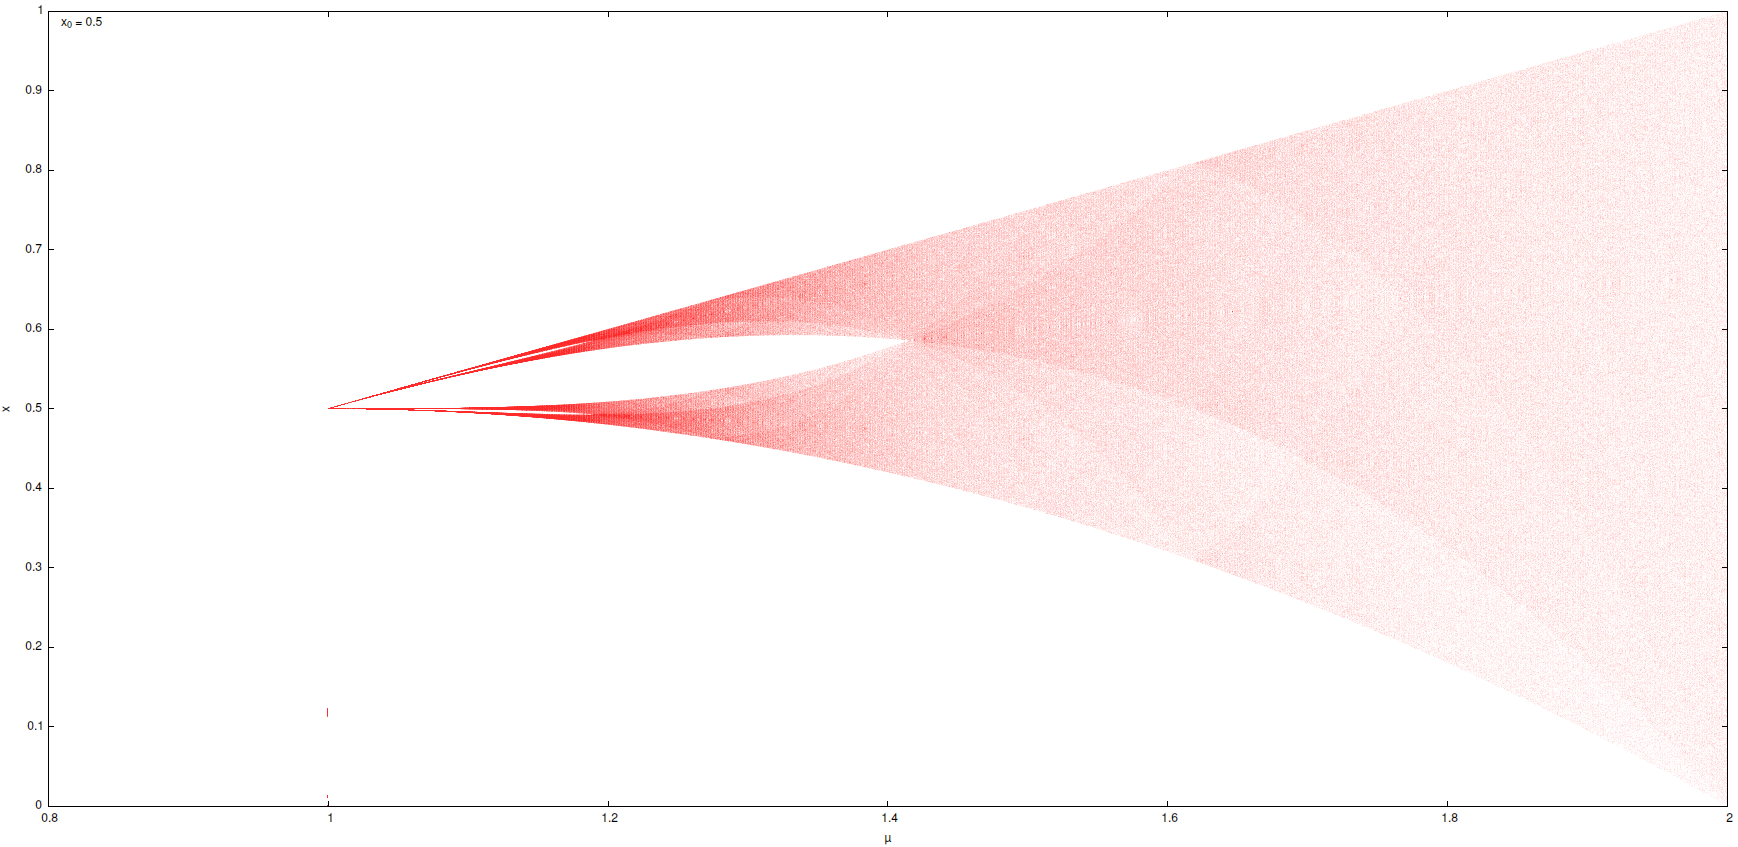
\includegraphics[width=0.8\linewidth]{Images/map5.png}
    \captionof{figure}{Diagrama de bifurcació de la iteració $f_\mu(x)=\begin{cases}
          \mu x    & x\in[0,1/2] \\
          \mu(1-x) & x\in[1/2,1]
        \end{cases}$ començant en $x=0.5$}
  \end{minipage}
\end{center}

\newpage

\section{\texorpdfstring{$\boldsymbol{f_\mu(x)=\mu x\exp{-\mu x-1}\quad x\in[0,\infty), \mu\in[0,\infty)}$}{f6}}
A la següent taula mostrem els valors aproximats de $\mu_k$ i $\lambda_k$ per a valors de $k$ petits:
\begin{table}[ht]
  \centering
  \begin{tabular}{c|c|c}
    $k$ & $\mu_k$   & $\lambda_k$ \\
    \hline
    \hline
    1   & 20.088691 & -           \\
    2   & 31.546168 & -           \\
    3   & 38.719884 & 1.597147    \\
    4   & 39.830118 & 6.461445    \\
    5   & 40.073241 & 4.566553    \\
    6   & 40.125549 & 4.647918    \\
  \end{tabular}
\end{table}

A més la primera vegada que apareixen els períodes 7, 5 i 3 són respectivament en $\mu = 47.453426$, $\mu= 50.204289$ i $\mu = 60.487693$.
Els gràfics següents mostren les aparicions d'alguns dels períodes així com el diagrama de bifurcació de la funció.
\begin{figure}[ht]
  \begin{subfigure}[ht]{0.45\linewidth}
    \centering
    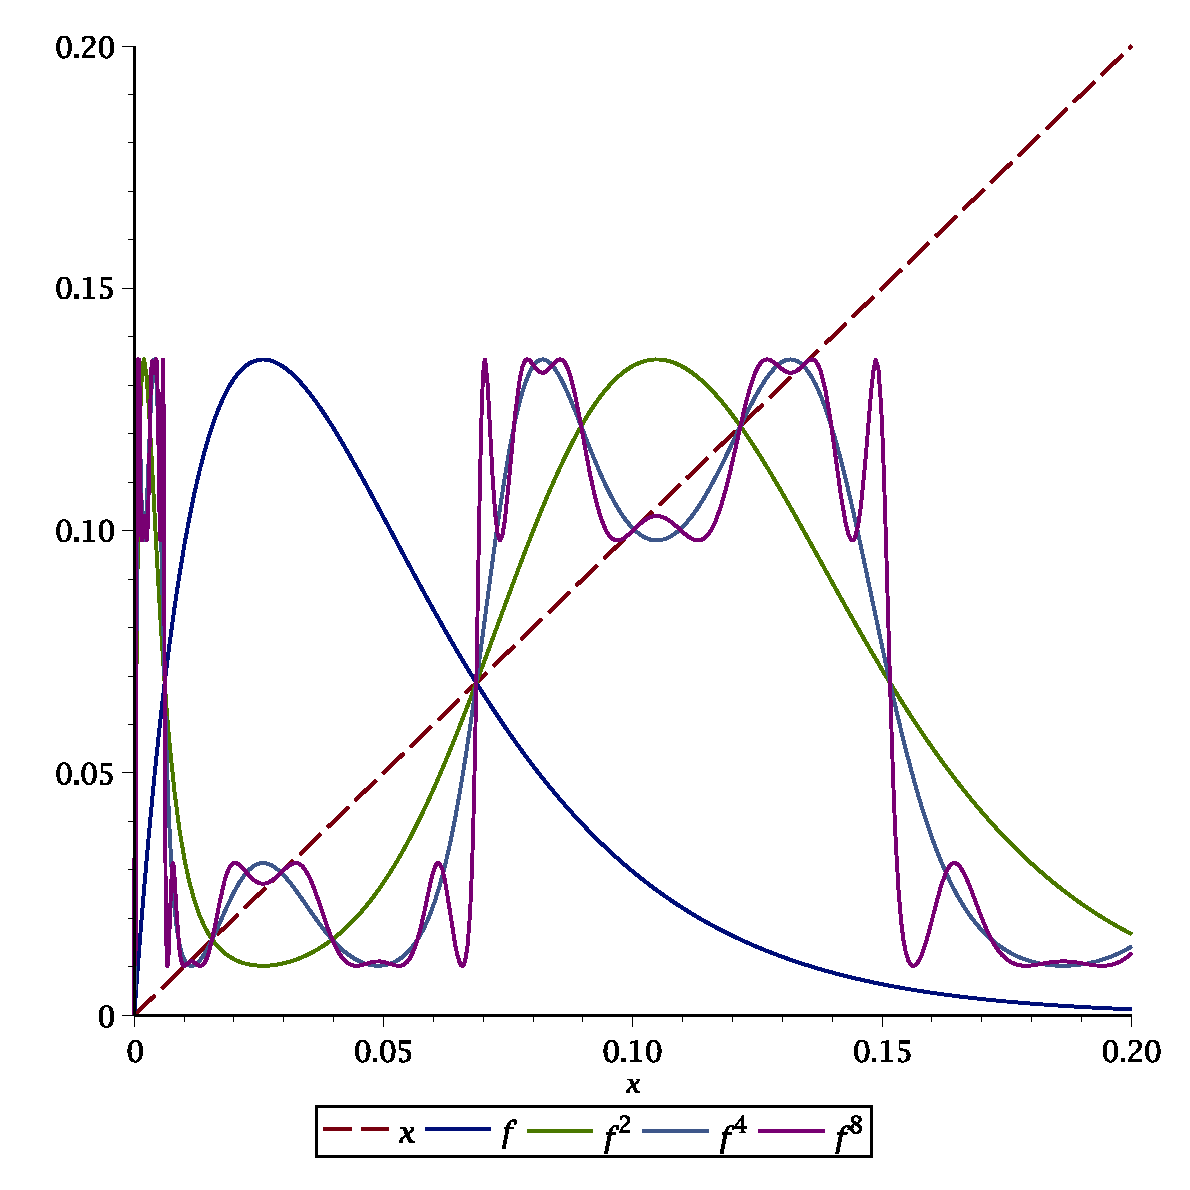
\includegraphics[width=\linewidth]{Images/map62.eps}
    \caption{Aparició del període 8}
  \end{subfigure}
  \hfill
  \begin{subfigure}[ht]{0.45\linewidth}
    \centering
    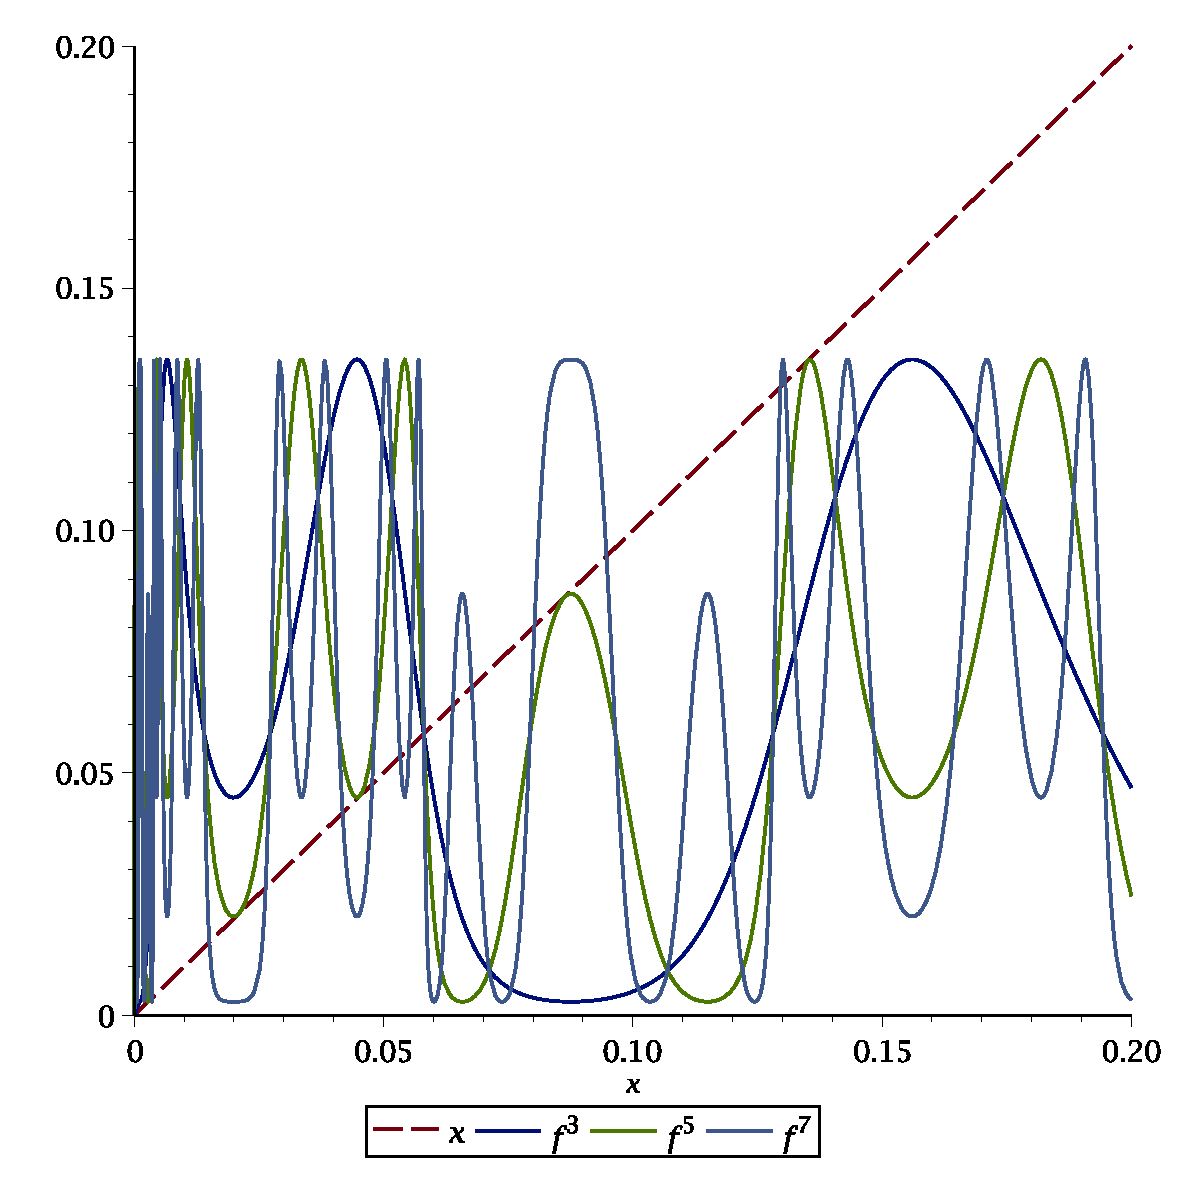
\includegraphics[width=\linewidth]{Images/map65.eps}
    \caption{Aparició del període 5}
  \end{subfigure}
\end{figure}
\begin{center}
  \begin{minipage}{\linewidth}
    \centering
    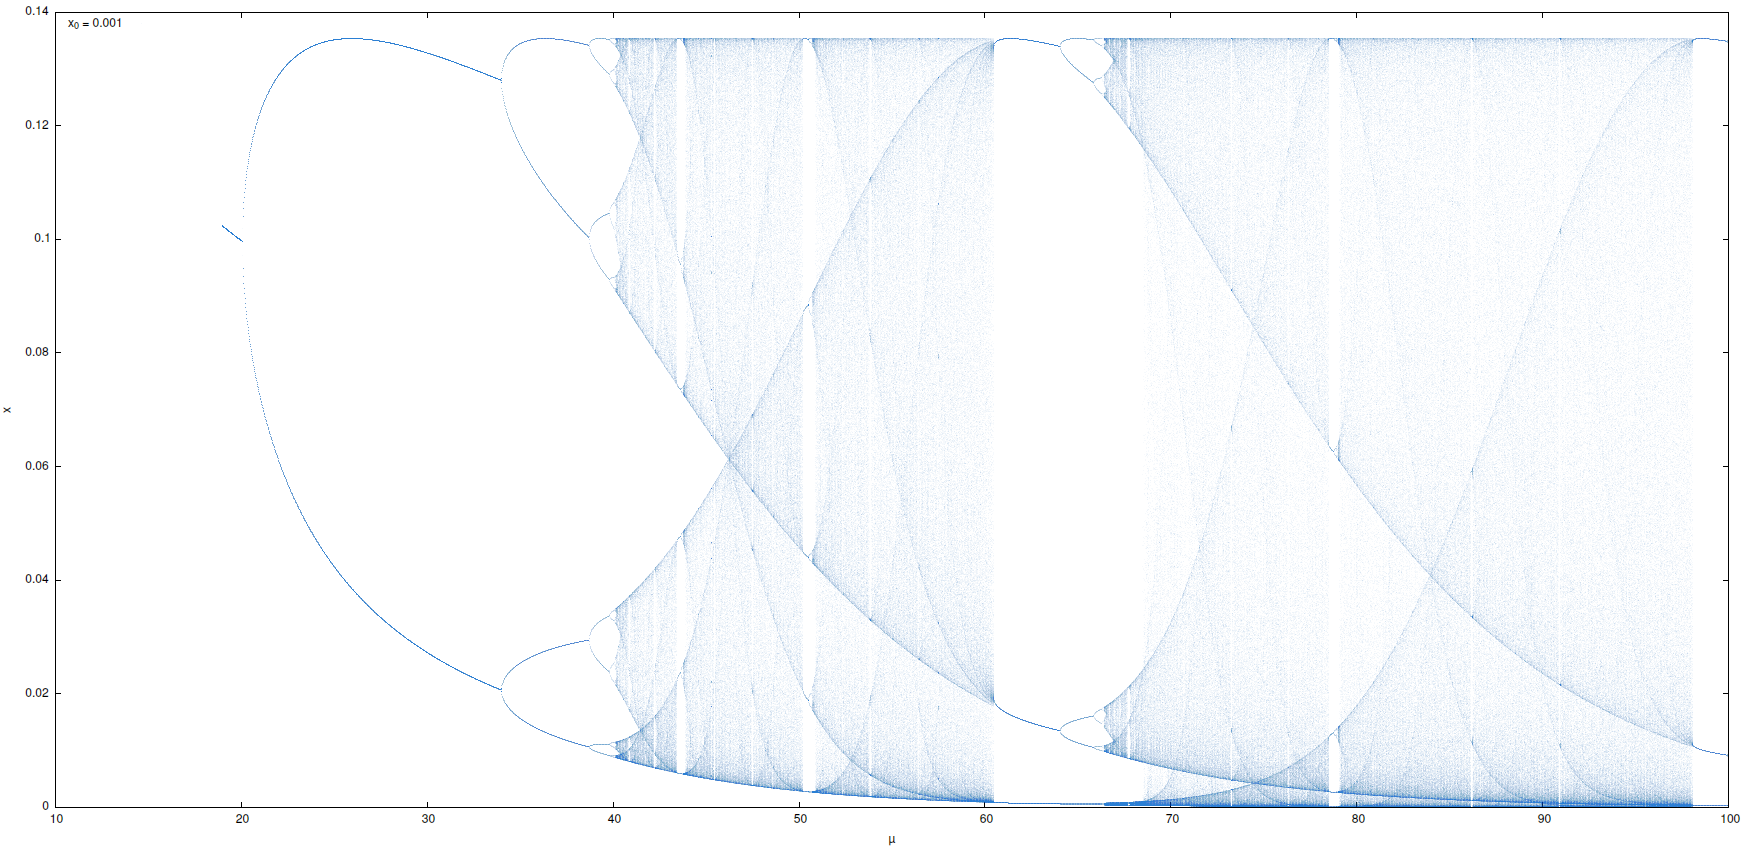
\includegraphics[width=0.8\linewidth]{Images/map6.png}
    \captionof{figure}{Diagrama de bifurcació de la iteració $f_\mu(x)=\mu x\exp{-\mu x-1}$ començant en $x=0.001$}
  \end{minipage}
\end{center}
\newpage
\section{Conclusions}
Al llarg d'aquesta pràctica he observat diverses coses que esmento a continuació. En primer lloc, el fet tractar-se d'un estudi numèric en problemes generalment mal condicionats ha fet que la precisió al obtenir les derivades no podia tenir més de 7 xifres significatives (usant precisió doble). Una primera solució que un podria pensar seria usar l'extrapolació de Richardson, que pretén millorar aquesta falta de precisió. Però en aquest cas tampoc acaba d'anar bé perquè l'error de les mesures ja ve implícit en el càlcul de les derivades, no en el fet de no poder fer l'increment espacial més petit per a calcular-les.

A més, com ens hem trobat ab la funció 5, el mètode de Newton no va bé per a funcions no diferenciables. La alternativa més raonable per una possible millora del treball seria fer una mena de bisecció en dues dimensions fent servir coneixements previs sobre el comportament de la funció a la qual volem calcular els zeros. Per exemple, d'aquesta sabem que en cada naixement d'òrbita periòdica, aquesta és atractora global, ja que totes les altres són repulsores. Amb aquesta informació i el fet que $\mu_{k+1}>\mu_k$ (i l'acotació superior d'aquestes per la $\mu$ on apareix el període 3) podríem anar recorrent aquest interval d'acotació i fent un estudi 1-dimensional en cada cas, per exemple amb el mètode de la bisecció. Aquesta solució tindria l'avantatge de no dependre de la diferenciabilitat de la funció.

Finalment, un fet remarcable és que en les funcions on hem pogut calcular més temres de $\mu_k$ (la 1 i la 4), hem observat que les $\lambda_k$ corresponents tenien el mateix límit $\lambda:=4.669201...$. Això ens porta a pensar que totes elles tenien de fet també aquest límit i que aquest només depèn de la geometria de la funció (totes les functions són unimodals).
\end{document}